\section{I/O Systems}

\paragraph{Device Management --- objectives}
\begin{itemize}
  \item \textbf{abstraction} from details of physical devices
  \item \textbf{uniform naming} that does not depend on hardware details
  \item \textbf{serialization} of I/O operations by concurrent applications
  \item \textbf{protection} of standard-devices against unauthorized accesses
  \item \textbf{buffering} if data from/to device cannot be stored in final destination
  \item \textbf{error handling} of sporadic device errors
  \item \textbf{virtualizing} physical devices via memory + time multiplexing
\end{itemize}

\paragraph{Device Management --- techniques}
\begin{itemize}
  \item \textbf{programmed I/O}: \\*
    $ - $ thread is busy-waiting for I/O operation to complete $ \to $ CPU cannot be used elsewhere \\*
    $ - $ kernel is \emph{polling} state of I/O device (command-ready, busy, error)
  \item \textbf{interrupt-driven I/O}: \\*
    $ - $ I/O command is issued \\*
    $ - $ processor continues executing instructions \\*
    $ - $ I/O device sends interrupt when command is done
  \begin{figure}[h]\centering\label{InterruptIO}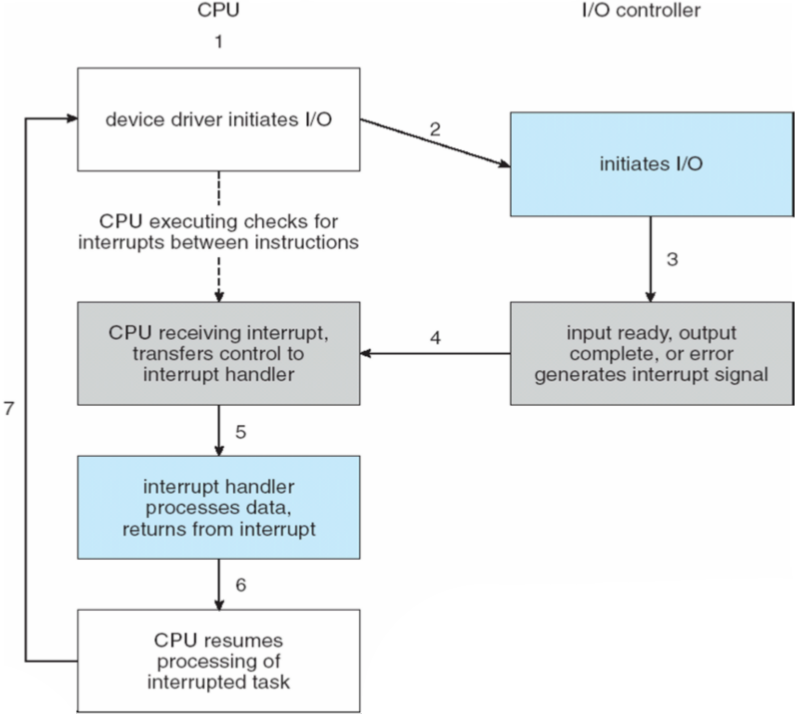
\includegraphics[width=0.33\textwidth]{InterruptIO}\end{figure}
  \item \textbf{direct memory access} (DMA): \\*
    $ - $ DMA module controls exchange of data between main memory and I/O device \\*
    $ - $ processor interrupted after entire block has been transferred \\*
    $ \to $ bypasses CPU to transfer data directly between I/O device and memory
  \begin{figure}[h]\centering\label{DMA}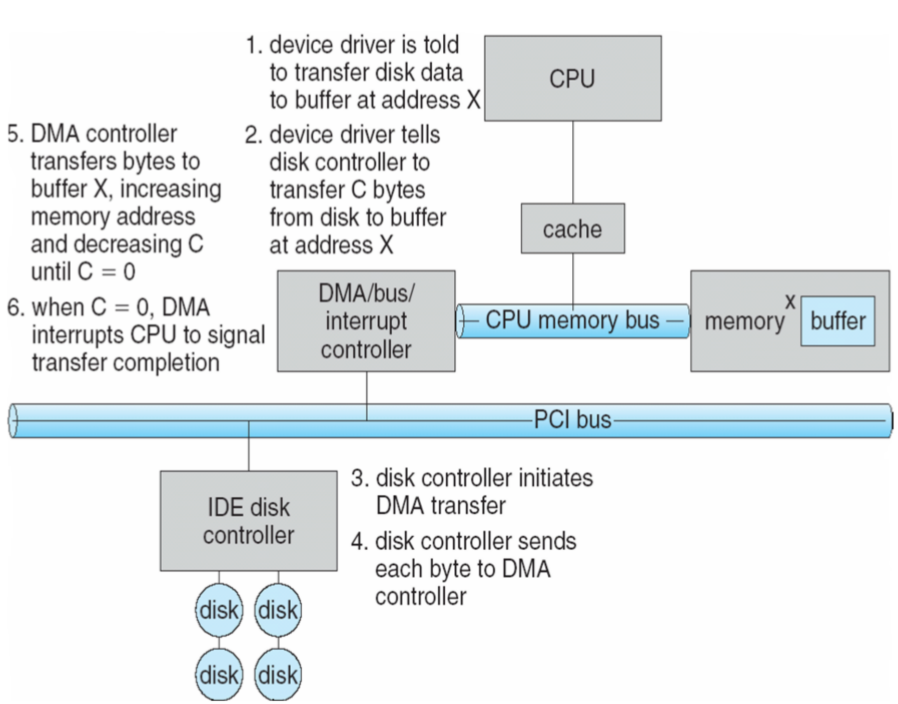
\includegraphics[width=0.33\textwidth]{DMA}\end{figure}
\end{itemize}

\paragraph{Kernel I/O Subsystem}
\begin{itemize}
  \item \textbf{scheduling}: order I/O requests in per-device queues
  \item \textbf{buffering}: store data in memory while transferring between devices
  \item \textbf{error handling}: recover from read/availability/write errors
  \item \textbf{protection}: protect from accidental/purposeful disruptions
  \item \textbf{spooling}: hold output to device if device is slow (e.g., printer)
  \item \textbf{reservation}: provide exclusive access for process
\end{itemize}

\paragraph{Device Drivers}
\begin{itemize}
  \item \textbf{jobs}: \\*
    $ - $ \emph{translate} user request through device-independent standard interface \\*
    $ - $ \emph{initialize} hardware at boot time \\*
    $ - $ \emph{shut down} hardware
\end{itemize}

\paragraph{Device Buffering}
\begin{itemize}
  \item \textbf{reasons}: \\*
    $ - $ without buffering threads must wait for I/O to complete before proceeding \\*
    $ - $ pages must remain in main memory during physical I/O
  \item \textbf{version 1 --- block-oriented}: \\*
    $ - $ information is stored in fixed-size blocks \\*
    $ - $ transfers are made a block at a time \\*
    $ - $ used for disks/tapes
  \item \textbf{version 2 --- stream-oriented}: \\*
    $ - $ transfer information as byte stream \\*
    $ - $ used for keyboard, terminals, \dots (most things that is not secondary storage)
\end{itemize}

\paragraph{Buffering --- user level}
\begin{itemize}
  \item \textbf{principle}: task specifies memory buffer where incoming data is placed
  \item \textbf{issues}: \\*
    $ - $ what happens if buffer is currently paged out to disk? $ \to $ data loss \\*
    $ - $ additional problems with writing? $ \to $ when is buffer available for re-use?
\end{itemize}

\paragraph{Buffering --- single}
\begin{itemize}
  \item \textbf{principle}: user process can process one data block while next block is read in
  \item \textbf{swapping}: can occur since input is taking place in system memory, not user memory
  \item \textbf{stream-oriented}: buffer = input line, carriage return signals end of line
  \item \textbf{block-oriented}: \\*
    $ - $ input transfers made to \emph{system buffer} \\*
    $ - $ buffer moved to \emph{user space} when needed \\*
    $ - $ another block read into system buffer
\end{itemize}

\paragraph{Buffering --- double}
\begin{itemize}
  \item \textbf{principle}: use 2 system buffers instead of 1 (per user process)
  \item user process can write/read from one buffer while OS empties/fills other buffer
\end{itemize}

\paragraph{Buffering --- circular}
\begin{itemize}
  \item \textbf{problem}: double buffer insufficient for high-burst traffic situations: \\*
    $ - $ many writes between long periods of computations \\*
    $ - $ long computation periods while receiving data \\*
    $ - $ might want to read ahead more than just single block from disk
\end{itemize}